\documentclass[a4wide, 10pt]{article}
\usepackage{a4, fullpage}
\usepackage[section]{placeins}
\usepackage{float}
\setlength{\parskip}{0.15cm}
\setlength{\parindent}{0cm}
\usepackage{graphicx}
\usepackage{caption}
\usepackage{subcaption}
\usepackage{amssymb}
\usepackage{amsmath}
\usepackage{hyperref}
\usepackage{graphicx,wrapfig,lipsum}
\begin{document}

\title{Maps, Sets and Fractals}

\section{Non Linear Maps - The Verhulst Pr}
Our initial approach to investigate this process was to depict the process iteratively 
 using a cobweb diagram. This was done in Matlab by plotting $x_{k+1}$ against
  $x_{k}$ for a number of iterations (1000) that was large enough to show any points where 
   the value of the function was tending to, the name of these points are called attractors.
    Moving between the range $ 0 \leq r < 2 $, you are able to see that there are specific
     values of r where the process changes from having $n$ attractors, say, to having $2n$
      attractors. At these $r$ values where the number of attractors doubles it is known as
       period doubling with period size $n$: 

%First 5 images       
\begin{figure}[H]
        \centering
        \begin{subfigure}[b]{0.19\textwidth}
                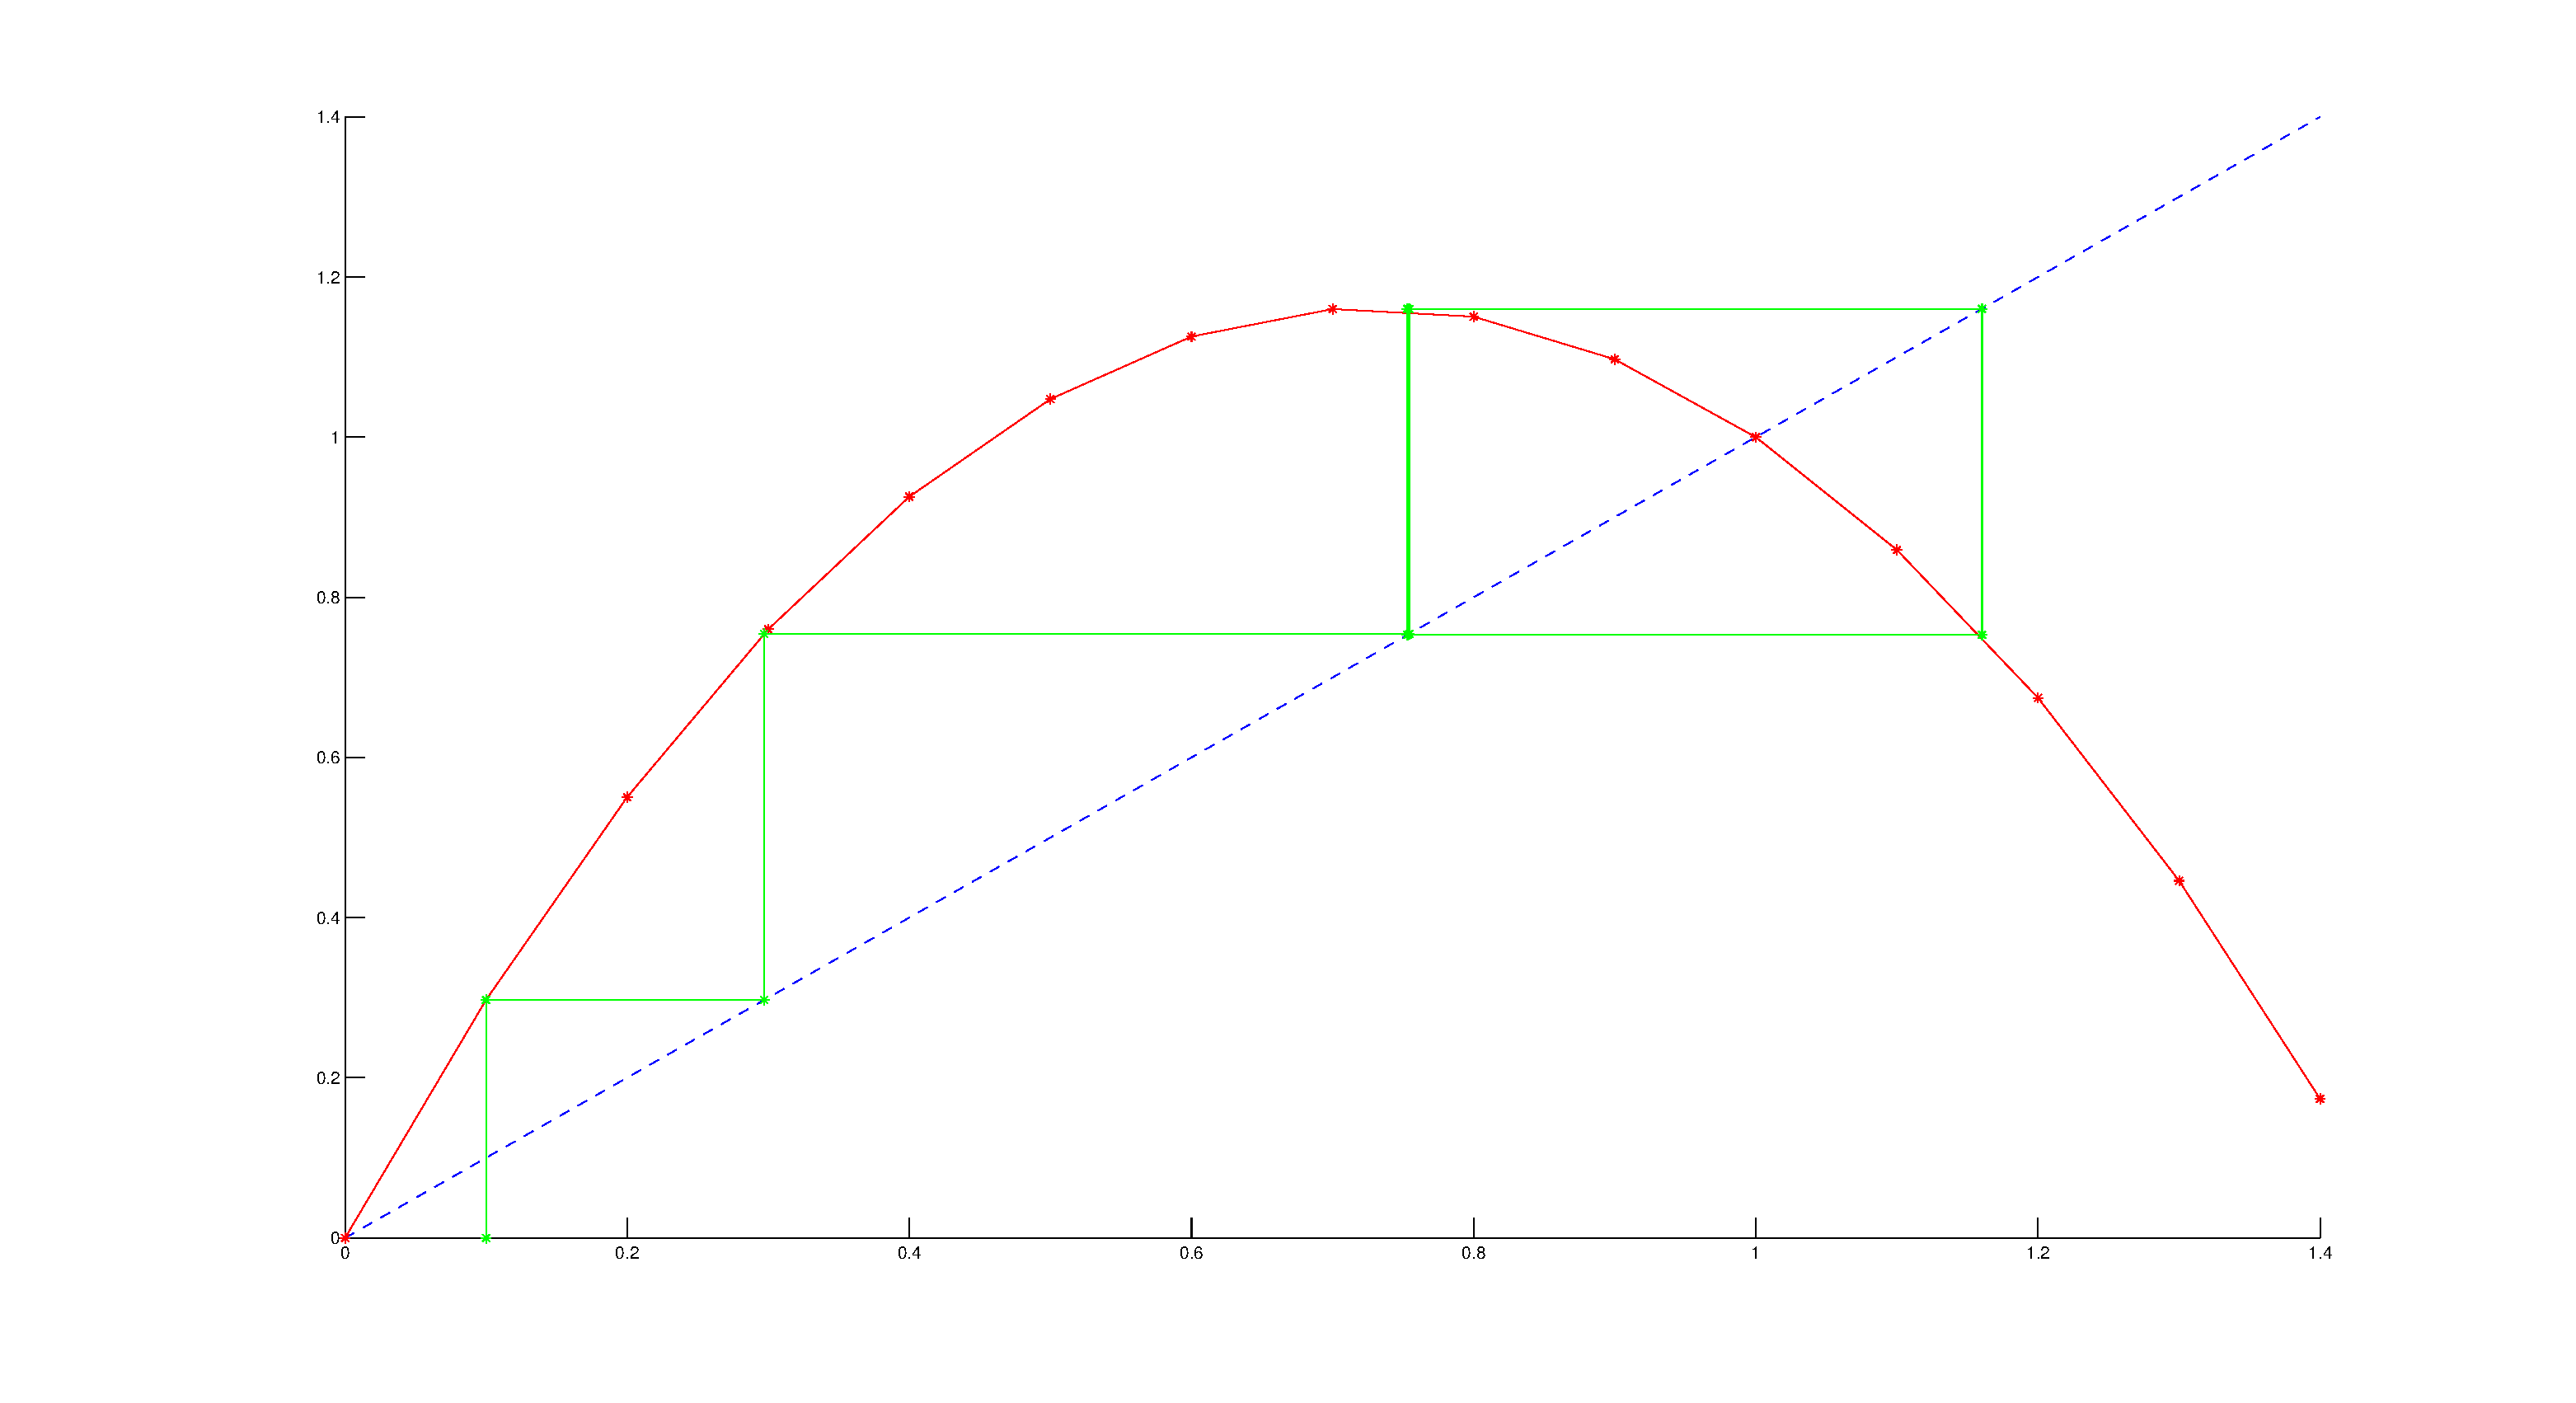
\includegraphics[width=\textwidth]{EPSFiles/CobwebPD_2_VMap}
                \caption{4 Attractors, \newline \hspace{2cm} r = 2.19}
                \label{fig:Cobweb2}
        \end{subfigure}
        \begin{subfigure}[b]{0.19\textwidth}
                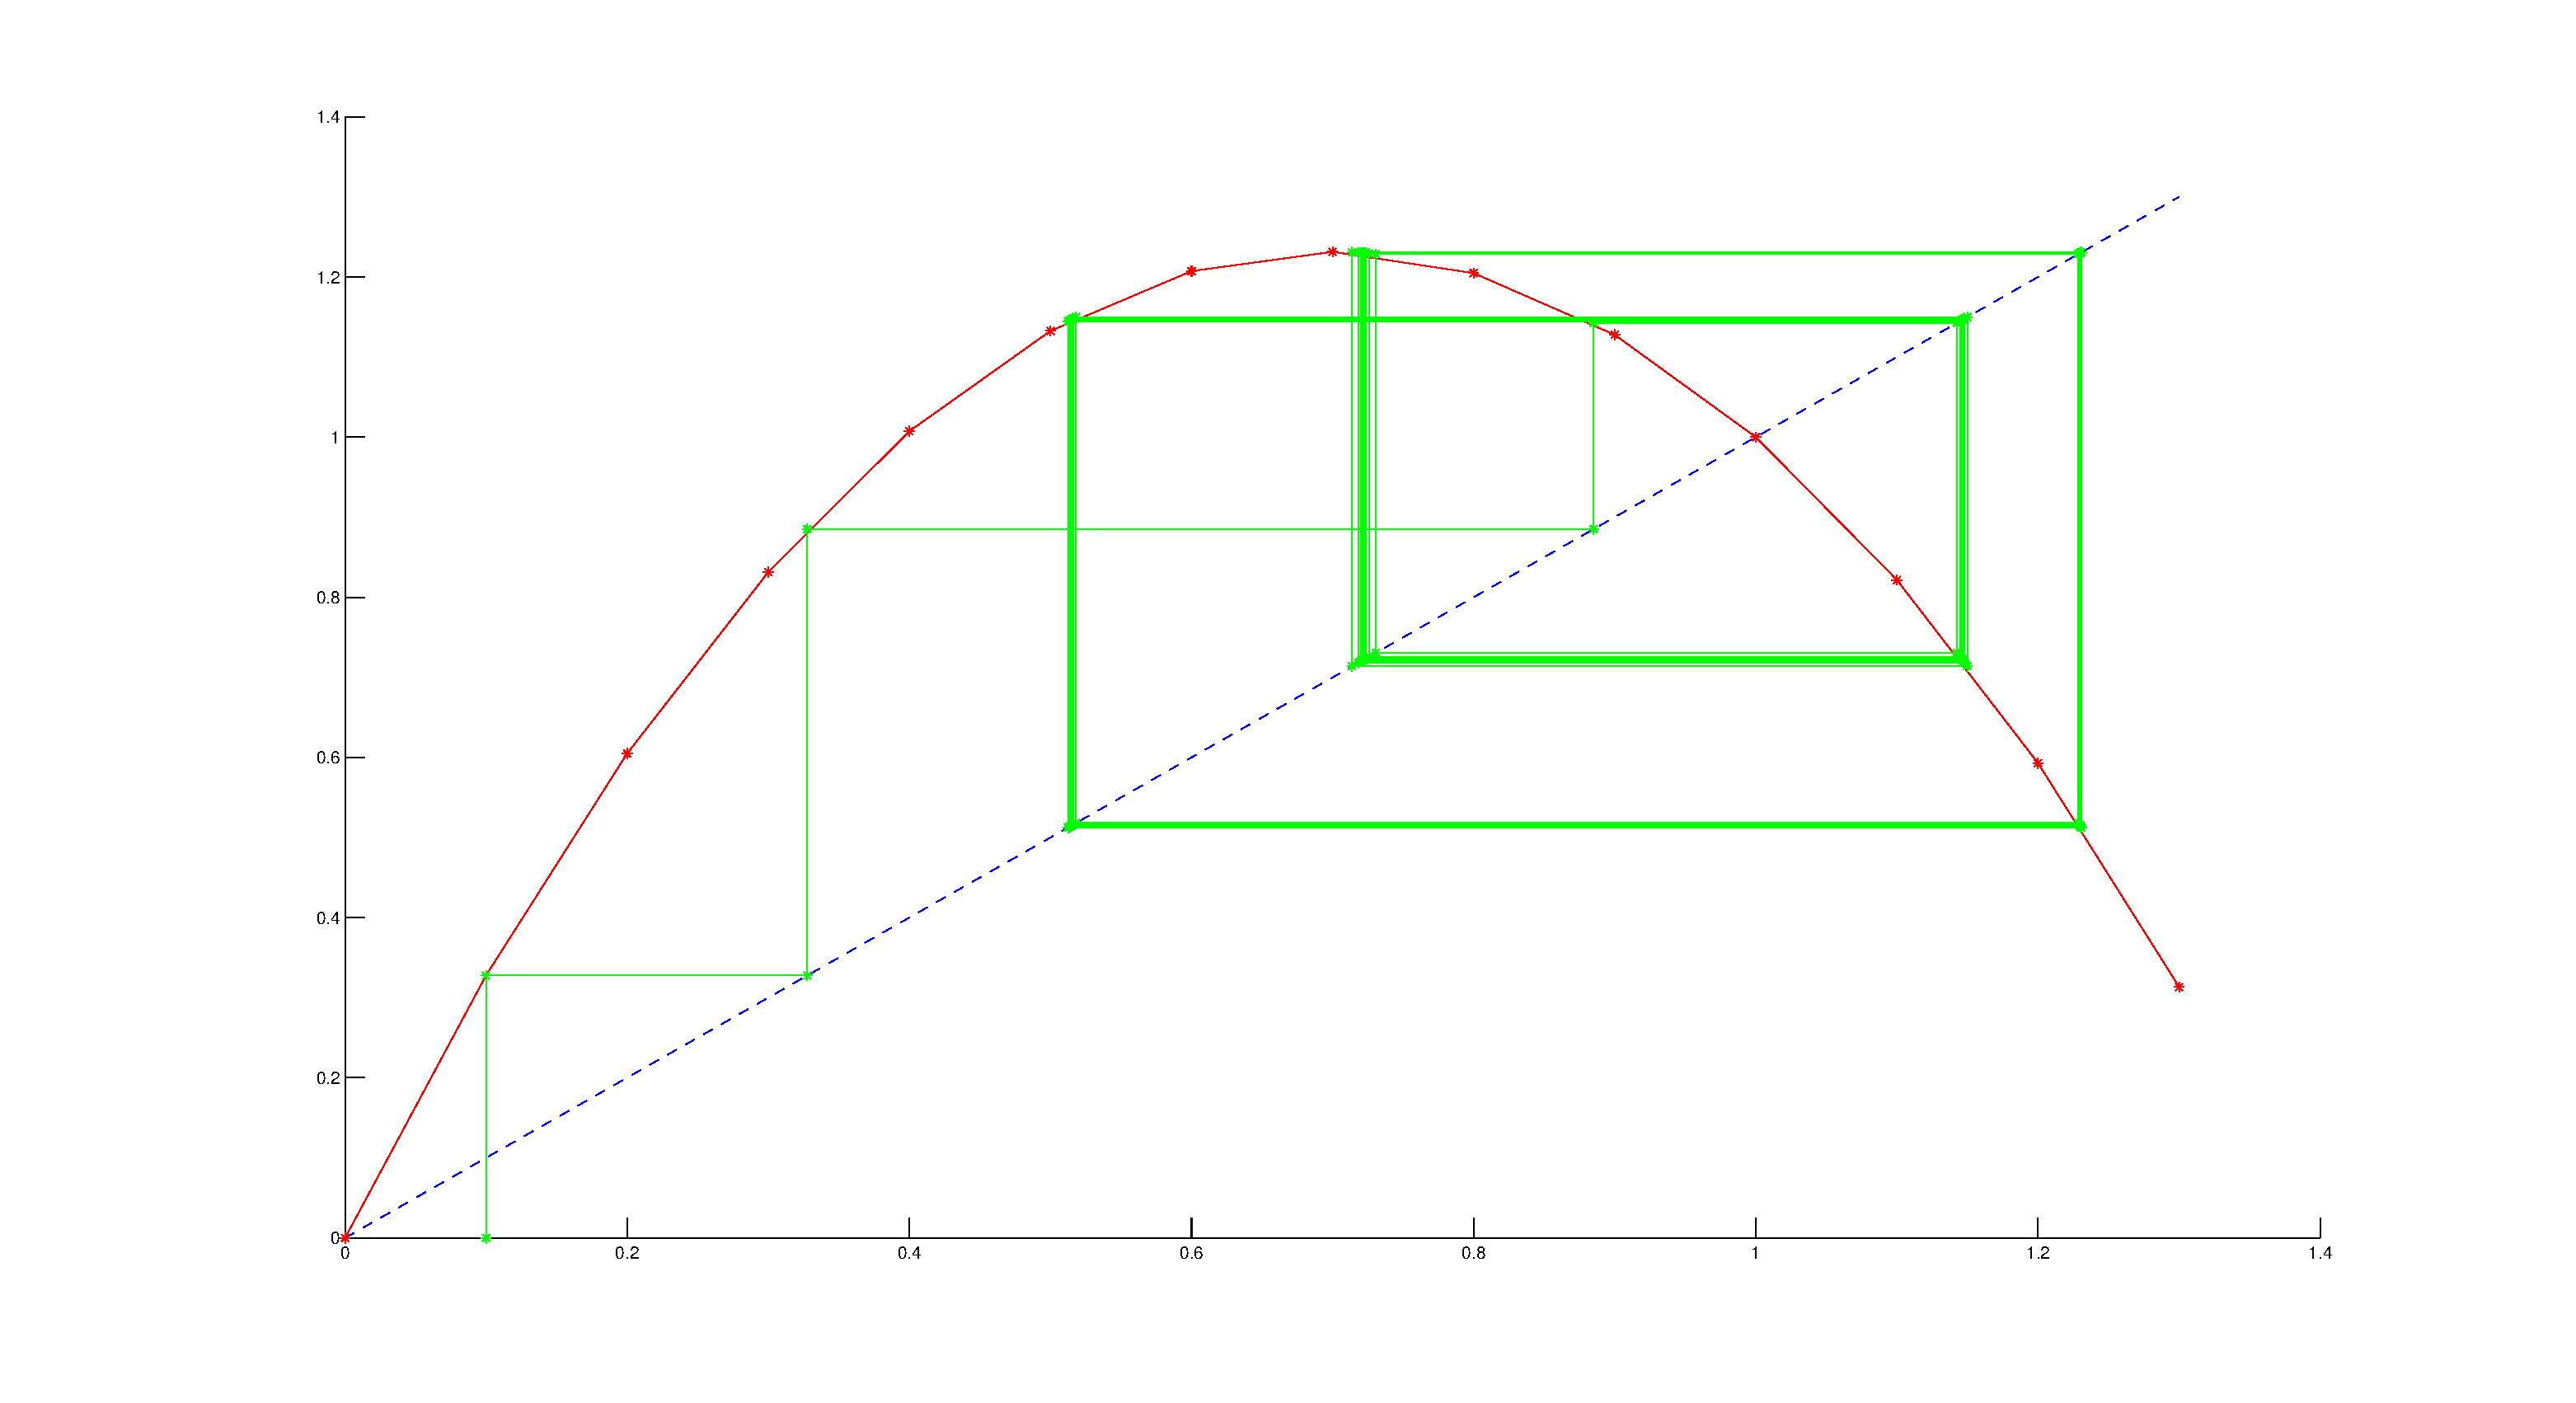
\includegraphics[width=\textwidth]{EPSFiles/CobwebPD_4_VMap}
                \caption{4 Attractors, \newline r = 2.53}
                \label{fig:Cobweb4}
        \end{subfigure}
        \begin{subfigure}[b]{0.19\textwidth}
                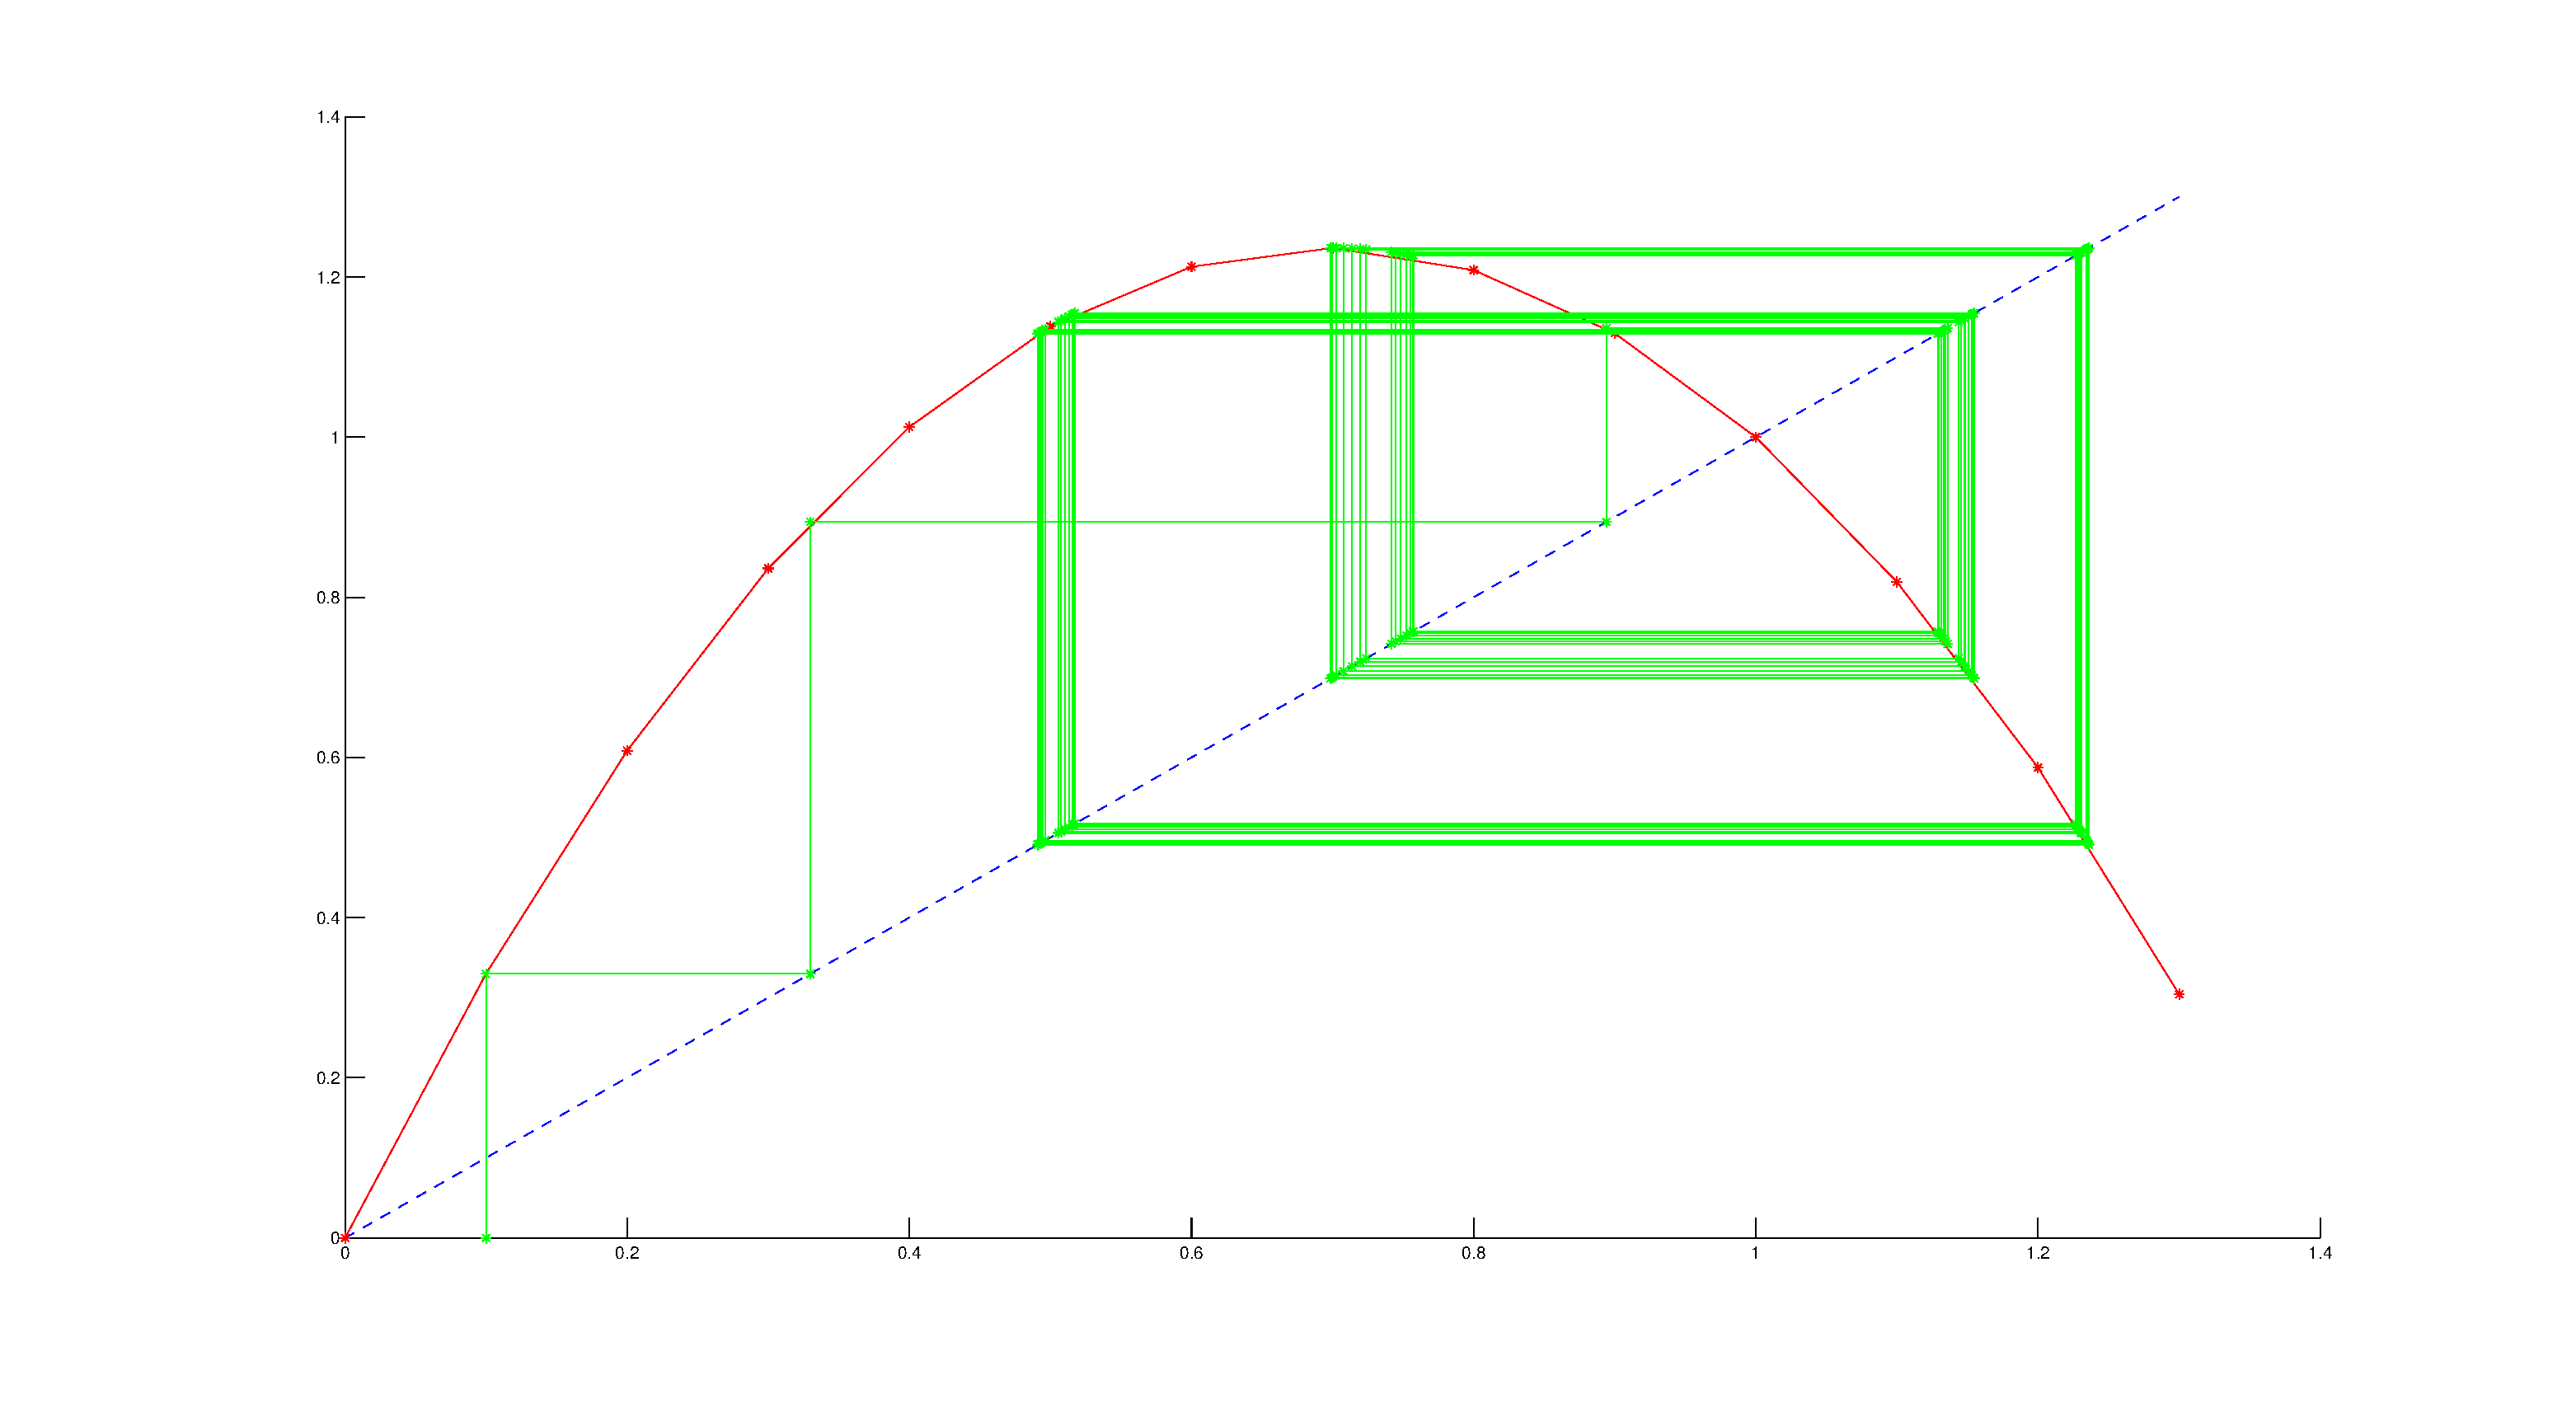
\includegraphics[width=\textwidth]{EPSFiles/CobwebPD_8_VMap}
                \caption{8 Attractors, \newline r = 2.553}
                \label{fig:Cobweb8}
        \end{subfigure}
        \begin{subfigure}[b]{0.19\textwidth}
                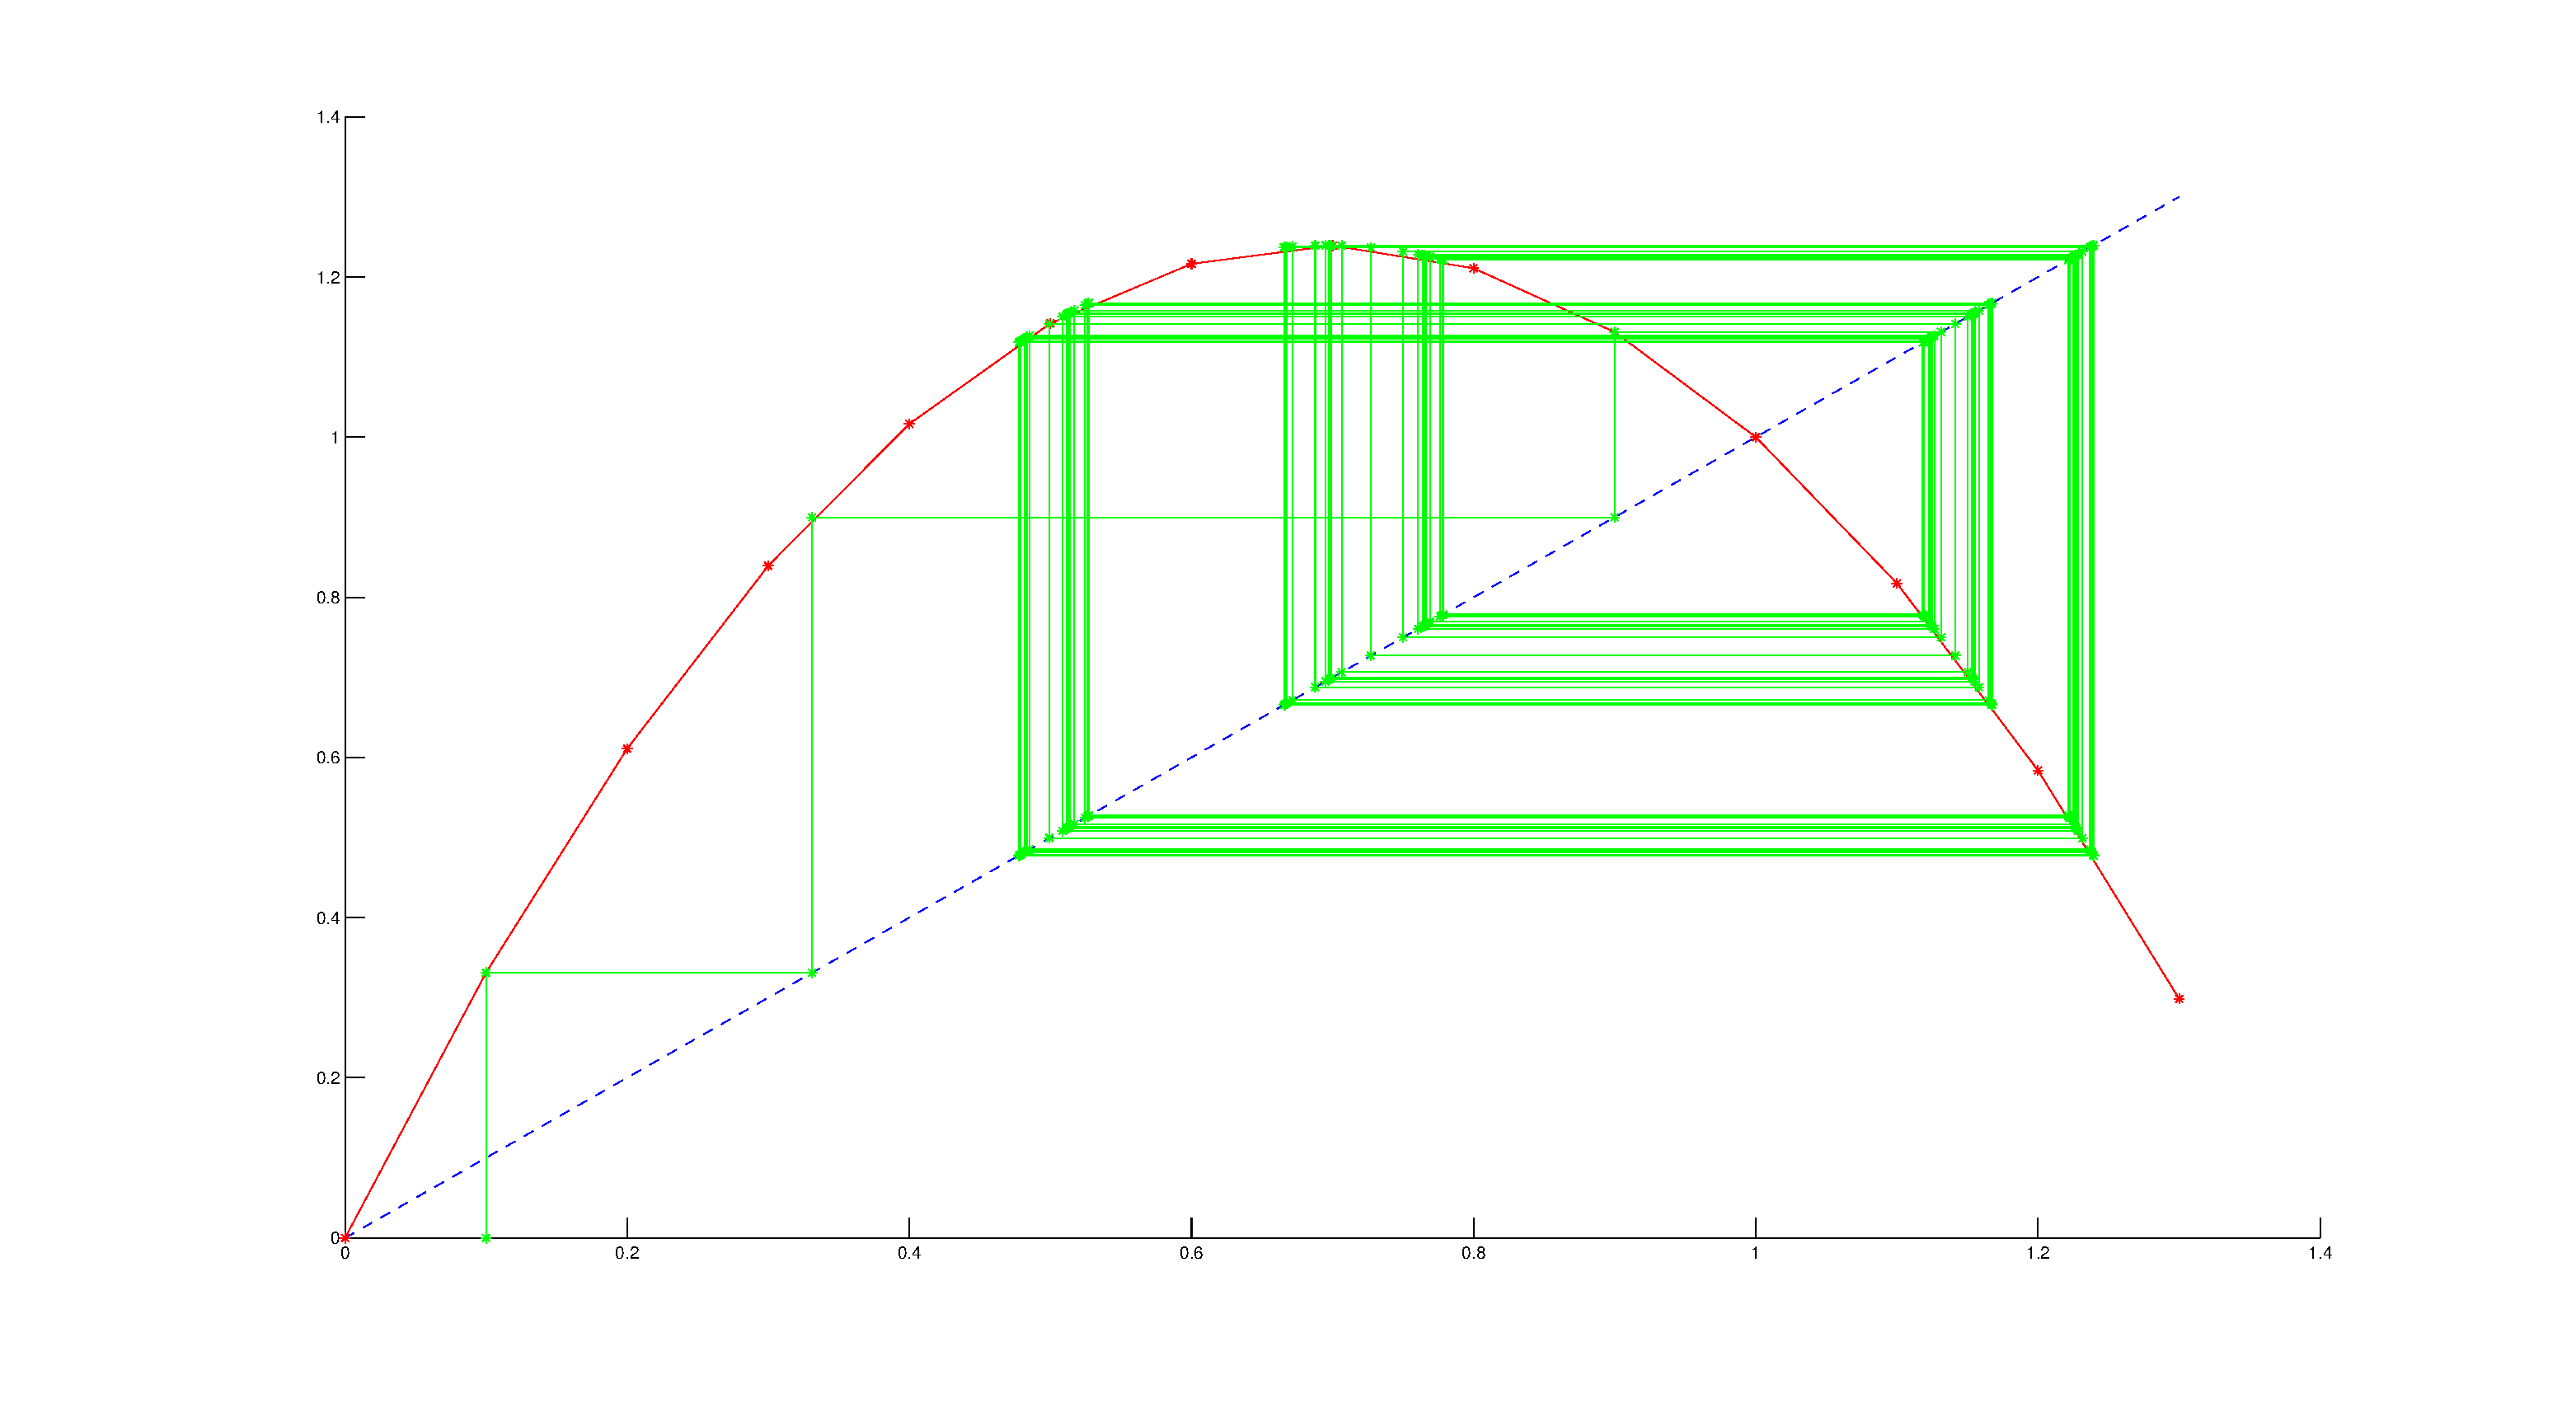
\includegraphics[width=\textwidth]{EPSFiles/CobwebPD_16_VMap}
                \caption{16 Attractors, \newline r = 2.568}
                \label{fig:Cobweb16}
        \end{subfigure}
        \begin{subfigure}[b]{0.19\textwidth}
                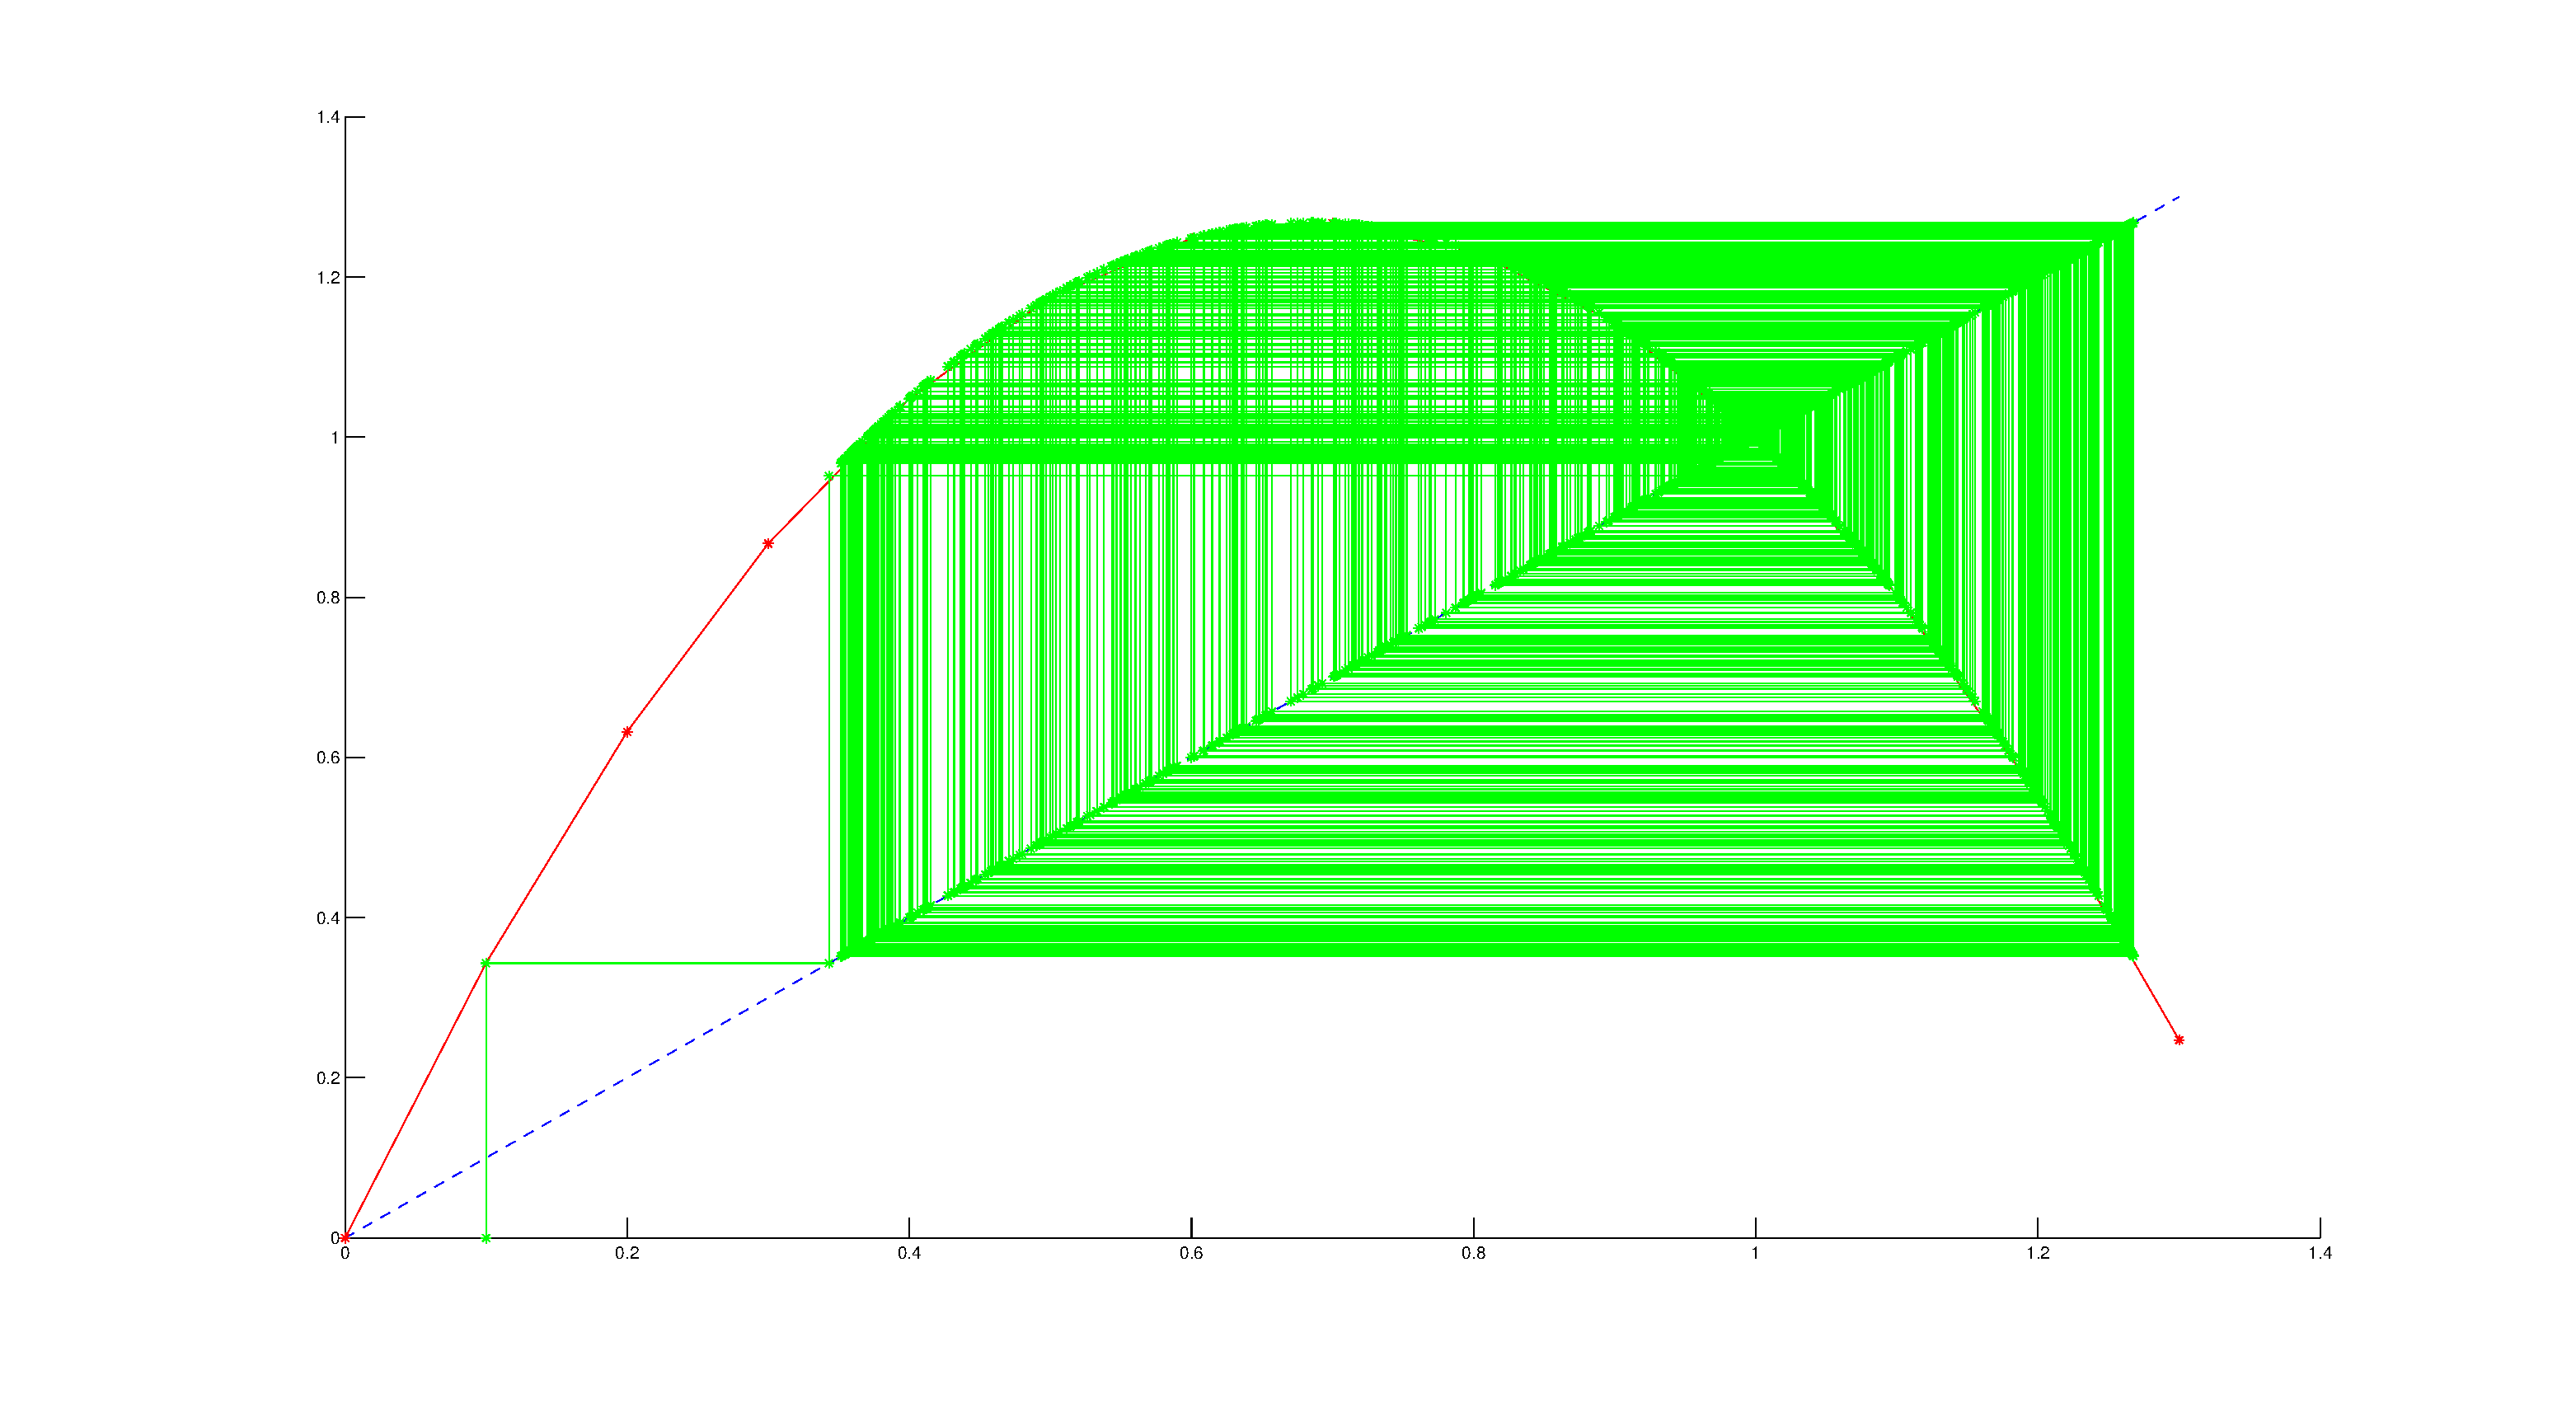
\includegraphics[width=\textwidth]{EPSFiles/CobwebPD_Random_VMap}
                \caption{Chaos, \newline r = 2.7}
                \label{fig:CobwebChaos}
        \end{subfigure}  
        \caption{Cobweb diagrams for Verhulst map with different $r \textrm{-values}$.}
\end{figure}

We found that different shaped orbits occurred at different r values corresponding to the number of
 period doubling points it has. You can see that a period double with two attractors shown in figure~\ref{fig:Cobweb2}
  looks like a rectangle orbit and a period double with four attractors in figure~\ref{fig:Cobweb4} is
   shown as two overlapping rectangles. When the amount of period doubling becomes quite large the shape of the
    orbits become more and more complex until it is hard to see  
     values being repeated and the orbit is filled with an infinite number of attractors scattered
      about the graph which depict a chaotic orbit. There still seems to be order amongst this chaos
       though.
 
The figure below is the result of plotting the points of the Verhulst map's $x_{k}$ values
 against the value of $r$ they were calculated at for $ 0 \leq r < 3 $. As you can see,  
  the graph seems to be covered up by lots of interweaving lines, however, looking closely,
   there seems to be a main pattern we are able to make out in the graph's ongoing structure.
    This figure shows the period doubling more clearly than the cobweb diagrams could.

\begin{figure}[H]

    \centering

    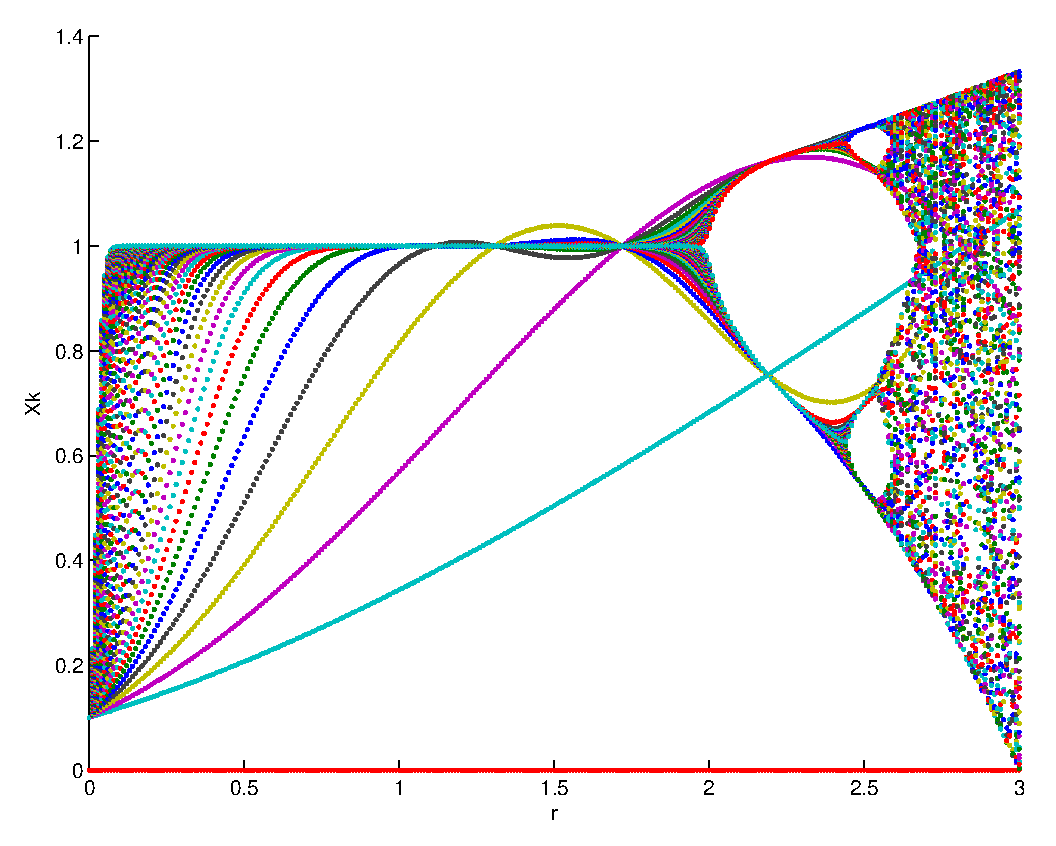
\includegraphics[scale=0.3]{EPSFiles/VerhulstAllXk}

    \caption{Verhulst map - plotting all iterations of $x_{k}$ against values of $r$ in range $0 \leq r < 3$.}
    \label{fig:VerhulstAllXk}

\end{figure}

The main pattern in the diagram above is therefore showing the value of the \emph{fixed points} in the
 Verhulst map for each $r$ value. Fixed points are the points that the map will converge to, if
  enough iterations are completed. These fixed points are also known
   as attractors, as mentioned before. The interweaving lines are simply the values of $x_{k}$ for
    very small k - before converging on the fixed points. Each colour in these figures corresponds to 
     a different iteration of $x_{k}$, so you can track what happens to each iteration as $r$ increases.

Period doubling becomes much clearer in the following two figures. The sequence of period doublings,
 or \emph{bifurcations}, as $r$ is varied is known as a \emph{period doubling cascade}. If the number
  of attractors at a given $r \textrm{-value}$ is \emph{n}, we say that there is a \emph{n-cycle
   attractor} for that value of $r$.

\begin{figure}[H]

    \centering

    \includegraphics[scale=0.3]{EPSFiles/VerhulstDots}

    \caption{Verhulst map with $ x_{0} = 0.1 $. $0 \leq r < 3$.}
    
    \label{fig:VerhulstDots}

\end{figure}

The figure above is created on Matlab by only plotting the values of $x_{k}$ for large $k$,
 thus getting rid of the interweaving lines shown in figure~\ref{fig:VerhulstAllXk}, which were caused by also plotting the $x_{k}$ for small $k$, when it hadn't
   converged on an attractor yet. In the above figure, only the final 32 iterations
    out of 10000 iterations of $x_{k}$ are plotted for each $r \textrm{-value}$. 

%It turns out that, for example, during a 2-cycle, the value of $x_{k}$ will oscillate between the 2
 %attractors, so odd iterations, i.e. $x_{1}$, $x_{3}$, etc., will all converge to one of the
  %attractors, and the even iterations will converge to the other one. This can be generalised to any n-
  %cycle, as consecutive iterations will go through attractor 1, then attractor 2, and so on, until
  % attractor $n$, which will be followed by attractor $1$, and then the pattern repeats itself\cite{Verhulst
  %  Map Period Doubling Information}. This idea is used in the code that finds the points where period
  %   doubling occurs, shown in the figure below.

%The point at $r = 0$ is due to the fact that, at $r = 0$, the equation simply
% becomes $x_{k + 1} = x_{k}$. Since the initial value for x was 0.1, in this case,
%  all iterations will give $x_{k} = 0.1$ when $r = 0$. 

The period doubling begins at $r = 2$, and after that, the distance between
 consecutive period doubling points on the $r \textrm{-axis}$ keeps decreasing. As
  $r$ increases to 2.57, this distance between consecutive period doubling points
   tends to 0. Eventually, at r = 2.57, there will be infinitely many attractors, so
    the value of each $x_{k}$ is essentially random\cite{Verhulst Map Period Doubling Information}. It is at this $r \textrm{-value}$
     that the Verhulst map descends into chaos. For $r > 3$, there are no attractors, 
      as $x_{k}$ now diverges for all $r \textrm{-values}$ above three.

This may all seem quite unexpected already - that such a simple equation can result
 in such a complex structure, simply by varying a single parameter. However, what is
  even more intriguing is the fact that inside the chaos, inside the \emph{randomness}, 
   order arises. Notice the point at about $r = 2.828$, there are 
    three attractors in the middle of the chaotic mess. This order doesn't last very long, and as
     $r$ increases, it quickly descends into chaos again, but the fact that it appears at all is
      extraordinary. 

%REFERENCE SOMETHING FROM GLEICK BOOK???

%TALK ABOUT HOW I DID THIS (On MATLAB)

\begin{figure}[H]

    \centering

    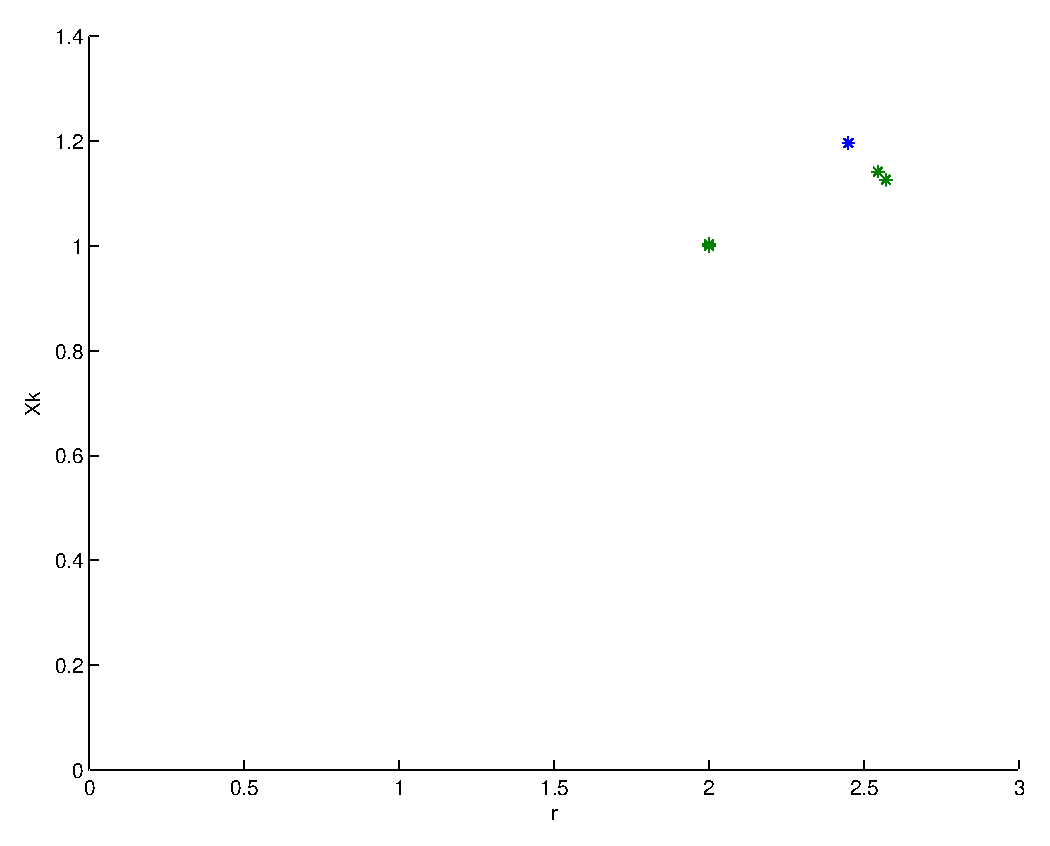
\includegraphics[scale=0.2]{EPSFiles/MAINVerhulstPointsEPS}

    \caption{The $r \textrm{-values}$ on the Verhulst map, from figure~\ref{fig:VerhulstDots}, where period doubling occurs.}
    
    \label{fig:VerhulstPoints}

\end{figure}

The figure above shows the first four values of $r$ where the period doubling occurs
 - 2, 2.449, 2.544, and 2.569. As you can tell, this is getting closer and closer to
  a particular number, namely 2.57, the point at which chaos occurs. Whilst analysing
   these points we found that the ratios of the differences between them also tended to a 
   	limit, this limit seemed close to the constant found by Mitchell Feigenbaum that occurs in
   	 many other non-linear maps\cite{Verhulst Map Period Doubling Information}. From the accuracy of the period doubling points we obtained, we didn't find exact convergence to the Feigenbaum constant, however the calculations below roughly show that the values of two ratios of differences are close to this constant. Finding more points of bifurcation would have given more accurate values for this ratio.	 
   	  
\begin{center} 	  
   	  $\frac{(2.449-2)}{(2.544-2.449)} = 4.726315$, $\frac{(2.544-2.449)}{(2.569-2.544)} = 3.8$ 
\end{center}
 
%FEIGENBAUM CONSTANT (Verhulst 2.57 google books- Feigenbaum's coming :P (Kiran))
At first we tried to create the figures in Matlab by always starting with $x_{0} = 0.1$, and then plotting the values of $x_{k}$
  when the number of iterations gets bigger than a certain value. This seemed to be time 
   consuming when we started making the interval between each consecutive $r \textrm{-value}$ smaller. It seemed 
    to be more efficient to create an array of values for large $x_{k}$ and then plot the whole 
     array against its' $r \textrm{-value}$ instead. 
       This method was carried through when making the plots for the other logistic maps. Other ways we 
 improved the figures for the non-linear maps were increasing the precision, by incrementing $r$ by a
  smaller amount so that the figure had more detail, and by making the array to store the iterations of
   $x_{k}$ large enough to store them all, rather than making a small array and having it increase in
    size every time it needed to be bigger, because this involved copying all contents of the array of
     size $n$ over to another array of size $n + 1$. Furthermore, we got rid of magic numbers by giving
      most parameters variable names, so that the figure can be easily improved or changed to be
       slightly different.
       
       
\end{document}